\chapter{Analisi}

\section{Descrizione e requisiti}

Il software mira alla costruzione di una versione virtuale del famoso gioco da tavolo “Monopoly”. 
Quest’ultimo è un gioco di società nel quale più giocatori a turno lanciano i dadi e muovono le proprie pedine su un tabellone 
composto da caselle; la maggior parte di queste sono proprietà: ovvero terreni acquistabili dai giocatori.
Lo scopo del gioco è di creare un monopolio, aumentando i beni o il denaro posseduto. 
Durante la partita i giocatori possono acquistare le proprietà capitandovi sopra e pagando una somma alla banca.
Una volta acquistate il giocatore potrà anche decidere se eventualmente migliorare le proprietà.
I giocatori si scambiano denaro a vicenda sotto 
forma di pagamenti. Quando un giocatore capita su una proprietà di un altro giocatore è costretto a pagare
a questo una somma di denaro. 
L’obiettivo è mandare gli altri giocatori in bancarotta, vince l’ultimo giocatore rimasto. 
Il software permetterà di creare e giocare un partita con un determinato numero di giocatori dallo 
stesso terminale.



\subsection*{Requisiti funzionali}
\begin{itemize}
    \item Il gioco potrà essere giocato su uno stesso dispositivo da un minimo di 2 giocatori ed un massimo di 6. L'utente
    potrà impostare altre opzioni di configurazione relative al gioco prima di avviare la partita.
	\item Il giocatore potrà tirare i dadi per far muovere la propria pedina sul tabellone.
	\item Durante il proprio turno ciascun giocatore avrà la possibilità di acquistare la proprietà sulla quale 
    si trova la sua pedina, se questa non appartiene a nessuno. Se la proprietà è già in possesso di un altro gicoatore 
    al giocatore che vi capita sopra verrà data la possibilità di pagare l’affitto al giocatore proprietario.
    \item Sul tabellone saranno presenti delle caselle speciali con effetti specifici sulla partita. Quando un giocatore 
    capita su una di queste caselle speciali l'effetto di quest'ultima si attiverà.
    \item Nel corso della partita un giocatore, quando capita sulle sue proprietà, le potrà migliorare spendendo
    del denaro per posizionare delle case che elevano il costo dell’affitto.
    \item Durante il proprio turno, se lo desidera, il giocatore potrà vendere alla banca 
    proprietà, o eventuali case presenti su esse, precedentemente acquistate.
\end{itemize}


\subsection*{Requisiti non funzionali}
\begin{itemize}
    \item 
    Monopoly dovrà permettere agli utenti di aggiungere e 
    modificare gli effetti speciali del gioco in facilità e senza toccare il codice
    \item \b NON LO INSERIREI \b salvare su file lo storico dei risultati delle partite precedenti
    \item Monopoly potrà essere giocato attraverso un'interfaccia grafica
    che dovrà essere in grado di adattarsi alle dimensioni di vari schermi
    \item 
    Monopoly dovrà permettere agli utenti di alterare in facilità la 
    configurazione del gioco (impostazioni della partita, struttura del tabellone e caselle che lo compongono)
    \item \b NON LO INSERIREI \b rendere l’applicazione portabile su più SO
\end{itemize}

\section{Modello del dominio}
Nella versione da tavolo del gioco, solitamente sono i giocatori a coordinarsi tra di loro
nella rotazione dei turni e nel controllare se un compagno di gioco ha perso e va dunque eliminato dalla partita.
Questo aspetto del gioco può risultare anche confusionario alle volte, soprattutto in situzioni particolari come ad esempio
nel caso in cui un giocatore finisce in prigione e deve rimanerci per un determinato numero di turni e le azioni che può
svolgere nel suo turno cambiano. 
Per modellare questo aspetto è stata inserita un'entità esterna che chiameremo arbitro (referee). All'arbitro sono delegate
tutte le operazioni di coordinazione del gioco e dei suoi partecipanti. 
Queste operazioni sono:
\begin{itemize}
    \item
    Coordinare il turno dei giocatori concedendogli di giocare, e permettendogli di terminare il turno solo se hanno svolto tutte le
    azioni obbligatorie
    \item 
    Decretare se un giocatore è eliminato oppure no sulla base della sua situazione finanziaria,
    se il saldo del portafoglio del giocatore è in negativo perde la partita e tutti i suoi contratti di proprietà
    ritornano alla banca, disponibili per l’acquisto. 
    \item
    Decretare se il gioco è finito e chi è il vincitore
\end{itemize}
Come è stato detto, a ogni giocatore (Player) viene concesso periodicamente dall'arbitro il proprio turno d’azione sulla base di una rotazione ciclica.
Durante il suo turno il giocatore muove sul tabellone (Board) la propria pedina (Pawn) tirando dei dadi (Dices).
Il tabellone è composto da una serie di caselle (Tile) disposte in un percorso ciclico. Il giocatore muove la propria pedina saltando 
un numero di caselle corrispondenti al suo tiro del dado e atterrando su una nuova casella. 
Questa casella può essere una proprietà (Property) oppure una casella speciale (Special), 
e sulla base di ciò cambia radicalmente l’interazione dell’utente. 
Le proprietà sono caselle alle quali è associato un contratto di proprietà (Title deed). 
Quando un giocatore capita su una casella di tipo proprietà non ancora in possesso di nessun altro può richiedere alla banca (Bank) di acquistare
il relativo contratto di proprietà (Title deed) associato alla suddetta proprietà.
Il giocatore paga una somma alla banca e gli viene consegnato il contratto, da questo momento in poi il giocatore possiede la proprietà.
Il contratto di proprietà è un documento che descrive tutte le informazioni monetarie relative alla proprietà come il prezzo d'acquisto,
prezzo di vendita e le varie opzioni di affitto, il loro costo e le condizioni di applicabilità.
La banca possiede tutti i contratti non acquistati.\newline
Se invece la proprietà su cui è capitato il giocatore era già stata comprata in precedenza da un altro giocatore allora si 
deve pagare l'affitto al proprietario. I giocatori, controllando il contratto di proprietà, concorderrano a quanto ammonta la somma di denaro.
Se in un turno successivo all'acquisto il giocatore ricapita su una casella di sua proprietà può decidere se migliorarla aggiungendo case 
o alberghi pagando dei soldi alla banca.
Infine ogni giocatore può rivendere alla banca un contratto di proprietà e ricevere del denaro in cambio.
Ogni giocatore ha associato un portafoglio (wallet) contente del denaro. Attraverso il suo portafoglio
il giocatore compie tutte le operazioni di compravendita che comportano un addebito o prelievo di denaro (comprare/vendere contratti, pagare affitti\dots)\newline
Se il giocatore invece capita su una casella speciale (special) si attiverà un effetto caratteristico della casella (Effect)
che avrà ripercussioni sullo svolgimento del gioco 
(guadagno/perdita denaro, saltare un determinato numero di turni\dots). 
In particolare se si capita su una casella Imprevisti (Unexpected) o Probabilità (Probability) l'effetto non 
è specifico della casella stessa, ma viene letto da un mazzo di carte effetto (Unexpected deck e Probability deck). 
Il giocatore pesca una carta (Card) da uno dei due mazzi, legge l'effetto della carta e lo attiva. \newline

Parte della difficoltà consisterà nel riadattare un dominio che non nasce intrinsecamente per un progetto software.
Monopoly infatti nasce come gioco da tavolo e questo si riflette in molte interazioni e funzionalità, che non sono pensate 
nell'ottica di un'architettura software (un esempio è quello dato all'inizio della sezione sulla coordinazione fra i giocatori e 
l'entità arbitro). Molte azioni nel gioco spesso comportano la comunicazione di più entità (l'arbitro decreta il vincitore sia sulla base dei 
contratti che possiede sia sul suo portafoglio, migliorare una
proprietà ha come conseguenza un cambiamento sulla casella ma per attuarlo il giocatore deve interagire con la banca facendo riferimento
al contratto di proprietà, un giocatore può passare il turno solo se ha fatto determinate azioni che dipendono non solo dalla casella in cui
si trova ma anche dal suo contratto\dots). 
Sarà quindi difficile progettare un'architettura software che permetta di rappresentare il dominio del gioco
in maniera efficace e riadattabile. 


\begin{figure}[H]
    \centering
    \makebox[1.0\textwidth]{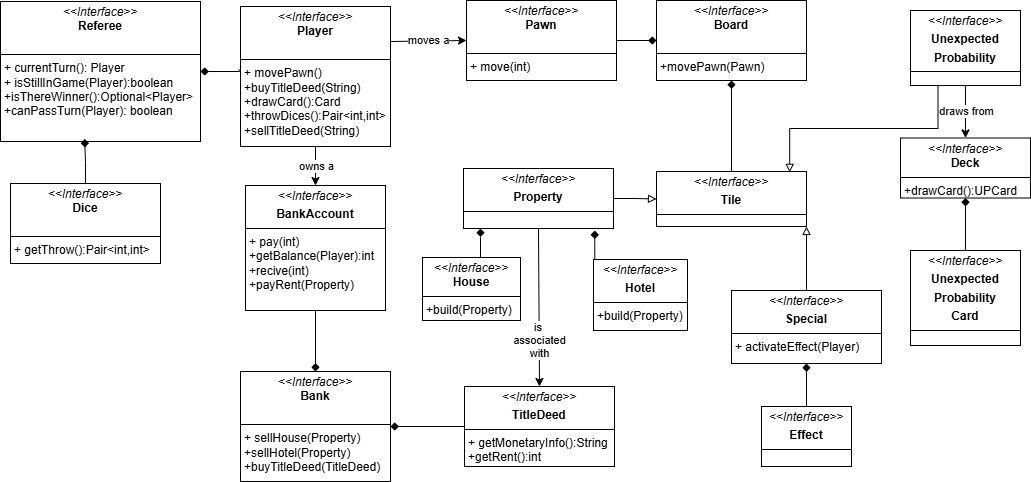
\includegraphics[width=1.3\textwidth]{img/entity_diagram.png}}	
    \caption{Schema UML dell'analisi del problema, con rappresentate le entità principali ed i rapporti fra loro}
	\label{img:entity_diagram}
\end{figure}
